\documentclass[jcp,twocolumn,longbibliography,superscriptaddress]{revtex4-2}
\usepackage{graphicx}
\usepackage[utf8]{inputenc}
\usepackage{amsmath}
\usepackage{verbatim}
\usepackage{amssymb}
\usepackage{listings}
\usepackage{color}
\usepackage{url}
\usepackage{hyperref}
\usepackage{amsmath}
\usepackage{mathtools}
\usepackage{xspace}
\usepackage{float}
\usepackage{multirow}
\usepackage[caption=false]{subfig}
\usepackage{xcolor}


\usepackage{ifxetex}
\ifxetex
\usepackage{fontspec}
\setmainfont[Mapping=tex-text]{STIXGeneral}
\else
\usepackage[T1]{fontenc}
\usepackage[utf8]{inputenc}
\fi

%\usepackage{caption}
\newcommand{\tvd}[1]{|| #1 ||_{\text{TV}}}
\newcommand{\tmix}[1][]{t_{\text{mix}}}
\newcommand{\tcorr}[1][]{t_{\text{corr}}}
\newcommand{\pit}[1]{\pi^{\{#1\}}}
\newcommand{\tvdt}[1]{\text{TVD}^{\{#1\}}}
\newcommand{\Ptrans}{\Phat^{\text{trans}}}
\newcommand{\Path}[1]{\PCAL_{#1}}
\newcommand{\Pres}{\Phat^{\text{res}}}
\newcommand{\MC}{\Pi}
\newcommand{\DISP}{\DCAL}
\newcommand{\DISPQ}{\DCAL_q}
\newcommand{\Ncards}{N_{cards}}
\newcommand{\cfirst}{c_{\text{first-n}}}
\newcommand{\ultranaive}{naive\xspace}
\newcommand{\fabulousformula}{rift-average expression\xspace}
\newcommand{\tchain}{\tau^{\text{chain}}}
\newcommand{\tsim}{\tau_{\text{sim}}}
\newcommand{\collisions}{\text{coll.}}
\newcommand{\Area}{V}
\newcommand{\MinArea}{V_0}
\newcommand{\swell}{homothetic\xspace}
\newcommand{\np}{non-periodic\xspace}
\newcommand{\HD}{\texttt{HistoricDisks}\xspace}
\newcommand{\piOne}{\pi^{(1)}}
\newcommand{\nunit}{\nhat_{\text{colls}}}
\newcommand{\nunitwallx}{\nhat_{\text{wall}}^{\pm \ehatvec_x} }
\newcommand{\nwallx}{n_{\text{wall}}^{\pm x} }
\newcommand{\nwallxy}{n_{\text{wall}}^{\pm \ehatvec_x \pm \ehatvec_y}}
\newcommand{\npair}{n_{\text{pair}} }
\newcommand{\vperp}{v^\perp}
\newcommand{\vperpwall}{\vperp_{\text{wall}}}
\newcommand{\vrelperp}{\Delta v^{\perp}} 
\newcommand{\vrelperppair}{\vrelperp_{ij}}
\newcommand{\aspect}[2]{\alpha\! =\! (#1 \! :  \! #2)}
\newcommand{\aspectclean}[2]{ (#1 \! :  \! #2)}
\newcommand{\RR}{R_v}
\newcommand{\scalfac}{\gamma}

\newcommand{\epsswell}{\epsilon_\alpha}
\newcommand{\rhox}{\rho^*_x}
\newcommand{\rhoy}{\rho^*_y}
\newcommand{\rhoxy}{\rho^*}
\newcommand{\delxmin}{\Delta x^{\min}}
\newcommand{\delxminij}{\delxmin_{ij}}
\newcommand{\delymin}{\Delta y^{\min}}
\newcommand{\wallcolls}[2][]{w:(#2 #1)}
\newcommand{\paircolls}{p:(ij)}
\newcommand{\simasymp}{\stackrel{N  \to  \infty}{\longrightarrow}}
\newcommand{\GDot}[2][]{\frac{\diff}{\diff t}G_{#2}^{\text{#1}}}

%\newcommand{\rhobotao}{\rho}
%\newcommand{\rhoxbotao}{\rho_x}
%\newcommand{\rhoybotao}{\rho_y}

%\newcommand{\colored}{} % Comment out for black version.
\ifdefined\colored
\newcommand{\revisionbl}[1]{{\color{red} #1}}
\newcommand{\revisionyn}[1]{{\color{red} #1}}
\newcommand{\revisionph}[1]{{\color{red} #1}}
\newcommand{\revisionlc}[1]{{\color{red} #1}}
\newcommand{\revisionacm}[1]{{\color{red} #1}}
\newcommand{\revisionwk}[1]{{\color{red} #1}}
\else
\newcommand{\revisionbl}[1]{{#1}}
\newcommand{\revisionyn}[1]{{#1}}
\newcommand{\revisionph}[1]{{#1}}
\newcommand{\revisionlc}[1]{{#1}}
\newcommand{\revisionacm}[1]{{#1}}
\newcommand{\revisionwk}[1]{{#1}}
\fi

%
% filename: latexcommands.tex
% version: 03-May-2018
%
\newcommand{\FIXME}[1]{{\bf FIXME \{}#1{\bf \}}}
%
% definition of float: algorithm
%
%
% Definitions for algorithms
%
\newcommand{\PROCEDURE}[1]{\textbf{procedure}\ \sub{#1}}
\newcommand{\CALL}[2][]{\textbf{call}\ \FUNCTION[#1]{#2} }
\newcommand{\FUNCTION}[2][]{\sub{#2} \glb #1 \grb }
\newcommand{\BRACE}[1]{
    \;\;\;  \left\{\begin{array}{l}#1\end{array} \right.}
\newcommand{\IS}[2]{#1 \leftarrow #2}
\newcommand{\SWAP}[2]{#1 \leftrightarrow #2}
\newcommand{\FOR}[1]{\textbf{for}\ #1 \textbf{: }}
\newcommand{\CHOICE}[1]{\textbf{choice}\SET{#1}}
\newcommand{\WHILE}[1]{\textbf{while } #1 \textbf{: }}
\newcommand{\ENDPROCEDURE}{\text{------} \\ \vspace{-0.8cm}}
\newcommand{\ENDPROCEDURET}{\text{------} \\ \vspace{-0.5cm}} % ENDPROCEDURE IN 
\newcommand{\GOTO}[1]{\textbf{goto}\ #1}
\newcommand{\CONTINUE}{\textbf{continue}}
\newcommand{\DO}{\textbf{do}}
\newcommand{\EXIT}{\textbf{exit}}
\newcommand{\BREAK}{\textbf{break}}
\newcommand{\TRUE}{\textbf{True}}
\newcommand{\IF}[1]{\textbf{if } #1 \textbf{: }}
\newcommand{\ELIF}[1]{\textbf{elif } #1 \textbf{: }}
\newcommand{\IFTHEN}[1]{\textbf{if (} #1 \textbf{) then}}
\newcommand{\ELSEIFTHEN}[1]{\textbf{else if (} #1 \textbf{) then}}
\newcommand{\IFELSE}[3]{\textbf{if (} #1 \textbf{) \{} #2 \textbf{\} else \{} #3
    \textbf{\}} }
\newcommand{\AND}{\text{and}}
%\newcommand{\AND}{\wedge} % not explicit enough
\newcommand{\OR}{\text{or}}
\newcommand{\SETPLUS}{\uplus}  % used in      SET \SETPLUS {j}
\newcommand{\THEN}{\textbf{then}}
\newcommand{\STOP}{\textbf{stop}}
\newcommand{\ELSE}{\textbf{else: }}
\newcommand{\ELSEIF}[1]{\textbf{else if } #1 \textbf{: then}}
\newcommand{\OUTPUT}[1]{\textbf{output}\ #1}
\newcommand{\PRINT}[1]{\textbf{print}\ #1}
\newcommand{\SORT}[1]{\text{sort[} #1\text{]}}
\newcommand{\INPUT}[1]{\textbf{input}\ #1}
\newcommand{\COMMENT}[1]{\text{\footnotesize (#1)}}
\newcommand{\TABLE}[1]{\{#1\}}
\newcommand{\LIST}[1]{\{#1\}}
\newcommand{\NULLLIST}{\LIST{0 \TO 0 }}
\newcommand{\SET}[1]{\{#1\}}
\newcommand{\EMPTYSET}{\{ \}}
\newcommand{\NULLSET}{\SET{0 \TO 0 }}
\newcommand{\sub}[1]{\texttt{#1}}
%
% definition of pi and complex unity
%
\newcommand{\mpi}{\uppi}
\newcommand{\mi}{\mathrm{i}}
%
% Definitions for text, equation numbers, figures, etc
%
\newcommand{\eq}[1]{eq.~\eqref{#1}}
\newcommand{\Eq}[1]{Eq.~\eqref{#1}}
\newcommand{\eqtwo}[2]{eqs~\eqref{#1} and~\eqref{#2}}
\newcommand{\Eqtwo}[2]{Eqs~\eqref{#1} and~\eqref{#2}}
\newcommand{\fig}[1]{Fig.~\ref{#1}}
\newcommand{\quot}[1]{``#1''}
\newcommand{\tab}[1]{Table~\ref{#1}} 
\newcommand{\chap}[1]{Chapter~\ref{#1}} 
\newcommand{\sect}[1]{Section~\ref{#1}} 
\newcommand{\alg}[1]{Algorithm~\ref{#1}} 
\newcommand{\algg}[1]{Alg.~\ref{#1}} 
\newcommand{\alggtwo}[2]{Algs~\ref{#1} and \ref{#2}} 
\newcommand{\lem}[1]{Lemma~\ref{#1}} 
\newcommand{\rem}[1]{Remark~\ref{#1}} 
\newcommand{\secttwo}[2]{Sections~\ref{#1} and~\ref{#2}} 
\newcommand{\SECT}[1]{\ref{#1}} 
\newcommand{\eg}{\textrm{e.g.}}
\newcommand{\cf}{\textrm{cf}}
\newcommand{\etc}{\textrm{etc.}}
\newcommand{\etcp}{\textrm{etc}}
\newcommand{\ie}{\textrm{i.e.}}
\newcommand{\vs}{\textrm{vs.}}
\newcommand\rmi[2]{\ensuremath{#1_\mathrm{#2}}}%

%
% text-indices
%
\newcommand{\betac}{{\beta_{\text{c}}}}  %  Critical inverse temperature
\newcommand{\Tc}{{T_{\text{c}}}}  %  Critical temperature
\newcommand{\Tr}{\text{Tr}}  %  Trace


%
%  non-diagonal density matrix , with optional parameter for `sym' `box' `cube' etc
%
\newcommand{\rhomat}[4][]{\rho^{\text{#1}\!}\lc #2,#3,#4\rc}
%
%
\newcommand{\dos}[2][]{\mathcal{N}^{#1} \! \glb #2 \grb} %  density of states
\newcommand{\dosa}[2][]{\mathcal{N}^{#1}_{#2}} %  density of states
\newcommand{\dosb}[2][]{\mathcal{N}^{#1} \! \glb #2 \grb} %  density of states
\newcommand{\dosc}[2][]{\mathcal{N}^{#1} \! \glc #2 \grc} %  density of states
%
\newcommand{\ACAL}{\mathcal{A}}  %  mathcal 
\newcommand{\BCAL}{\mathcal{B}}  %  mathcal
\newcommand{\CCAL}{\mathcal{C}}  %  mathcal%

\newcommand{\DCAL}{\mathcal{D}}  %  mathcal
\newcommand{\ECAL}{\mathcal{E}}  %  mathcal
\newcommand{\FCAL}{\mathcal{F}}  %  mathcal
\newcommand{\GCAL}{\mathcal{G}}  %  mathcal
\newcommand{\HCAL}{\mathcal{H}}  %  mathcal
\newcommand{\ICAL}{\mathcal{I}}  %  mathcal
\newcommand{\JCAL}{\mathcal{J}}  %  mathcal
\newcommand{\KCAL}{\mathcal{K}}  %  mathcal
\newcommand{\LCAL}{\mathcal{L}}  %  mathcal
\newcommand{\MCAL}{\mathcal{M}}  %  mathcal
\newcommand{\NCAL}{\mathcal{N}}  %  mathcal
\newcommand{\OCAL}{\mathcal{O}}  %  mathcal
\newcommand{\PCAL}{\mathcal{P}}  %  mathcal
\newcommand{\QCAL}{\mathcal{Q}}  %  mathcal
\newcommand{\RCAL}{\mathcal{R}}  %  mathcal
\newcommand{\SCAL}{\mathcal{S}}  %  mathcal
\newcommand{\TCAL}{\mathcal{T}}  %  mathcal
\newcommand{\UCAL}{\mathcal{U}}  %  mathcal
\newcommand{\VCAL}{\mathcal{V}}  %  mathcal
\newcommand{\WCAL}{\mathcal{W}}  %  mathcal
\newcommand{\XCAL}{\mathcal{X}}  %  mathcal
\newcommand{\YCAL}{\mathcal{Y}}  %  mathcal
\newcommand{\ZCAL}{\mathcal{Z}}  %  mathcal
%
\newcommand{\Abar}{\overline{A}}  %  overbar 
\newcommand{\abar}{\overline{a}}  %  overbar 
\newcommand{\Bbar}{\overline{B}}  %  overbar
\newcommand{\bbar}{\overline{b}}  %  overbar
\newcommand{\Cbar}{\overline{C}}  %  overbar
\newcommand{\cbar}{\overline{c}}  %  overbar
\newcommand{\Dbar}{\overline{D}}  %  overbar
\newcommand{\dbar}{\overline{d}}  %  overbar
\newcommand{\Ebar}{\overline{E}}  %  overbar
\newcommand{\ebar}{\overline{e}}  %  overbar
\newcommand{\Fbar}{\overline{F}}  %  overbar
\newcommand{\fbar}{\overline{f}}  %  overbar
\newcommand{\Gbar}{\overline{G}}  %  overbar
\newcommand{\gbar}{\overline{g}}  %  overbar
\newcommand{\Mbar}{\overline{M}}  %  overbar
\newcommand{\Nbar}{\overline{N}}  %  overbar
\newcommand{\Obar}{\overline{O}}  %  overbar
\newcommand{\Pbar}{\overline{P}}  %  overbar
\newcommand{\Qbar}{\overline{Q}}  %  overbar
\newcommand{\Rbar}{\overline{R}}  %  overbar
\newcommand{\Sbar}{\overline{S}}  %  overbar
\newcommand{\Tbar}{\overline{T}}  %  overbar
\newcommand{\tbar}{\overline{t}}  %  overbar
\newcommand{\Vbar}{\overline{V}}  %  overbar
\newcommand{\Xbar}{\overline{X}}  %  overbar
\newcommand{\xbar}{\overline{x}}  %  overbar
\newcommand{\Zbar}{\overline{Z}}  %  overbar
\newcommand{\zbar}{\overline{z}}  %  overbar
% the common Greek letters and their bold versions
%
\newcommand{\s}{\sigma}
\newcommand{\pitilde}{\tilde{\pi}}
\newcommand{\tautilde}{\tilde{\tau}}
\newcommand{\stilde}{\tilde{\sigma}}
\newcommand{\bs}{\boldsymbol{\sigma}}
\newcommand{\eps}{\varepsilon}
%
% poor man's bold for + and - (used for spins)
%
\newcommand{\minus}{\ensuremath{\pmb{-}}}
\newcommand{\plus}{\ensuremath{\pmb{+}}}
%
% max-zero abcd used for event rates.
%
\newcommand{\maxZeroa}[1]{\gla #1 \gra^+}   % maxzero ()
\newcommand{\maxZerob}[1]{\glb #1 \grb^+}   % maxzero ()
\newcommand{\maxZeroc}[1]{\glc #1 \grc^+}   % maxzero []
\newcommand{\maxZerod}[1]{\gld #1 \grd^+}   % maxzero {}


%
% Definition for { text } in equations (in columnar style)
%
\newcommand{\eqntexta}[1]{\!\!\!\mbox{\begin{tabular}{c}  #1 \end{tabular}}\!\!\! }
\newcommand{\eqntextb}[1]{\left(\!\!\!\mbox{\begin{tabular}{c}  #1 \end{tabular}}\!\!\! \right)}
\newcommand{\eqntext}[1]{\left\{\!\!\!\mbox{\begin{tabular}{c}  #1 \end{tabular}}\!\!\! \right\}}
%
% Definitions for display math
%
\newcommand{\BRA}[1]{\ensuremath{\langle #1 |}} % Dirac notation 
\newcommand{\BRAN}[1]{\ensuremath{\langle #1 }} % Dirac notation  Bra without |
\newcommand{\KET}[1]{\ensuremath{|#1 \rangle }} % Dirac notation
%
% exponentials with braces 'a': no brace 'b' () 'c' [] 'd' {}
%
\newcommand{\expa}[1]{\mathrm{e}^{#1}}   % high exponential groupings a
\newcommand{\expb}[1]{\exp \glb #1 \grb} % low exponential with groupings b
\newcommand{\expba}[1]{\exp \bigl( #1 \bigr)} % low exponential with groupings b-small
\newcommand{\expbb}[1]{\exp \Bigl( #1 \Bigr)} % low exponential with groupings b-medium
\newcommand{\expbc}[1]{\exp \biggl( #1 \biggr)} % low exponential with groupings b-large
\newcommand{\expbd}[1]{\exp \Biggl( #1 \Biggr)} % low exponential with groupings b-Xlarge
\newcommand{\expc}[1]{\exp \glc #1 \grc} % low exponential with groupings c
\newcommand{\expd}[1]{\exp \gld #1 \grd} % low exponential with groupings d
%
% ran functions 
%
\newcommand{\ran}{\texttt{ran}}
\newcommand{\rana}[2][]{\ran_{#1} \! \gla #2 \gra}  % ran-brace,  with - nothing
\newcommand{\ranb}[2][]{\ran_{#1} \! \glb #2 \grb}  % ran-brace,  with - nothing
\newcommand{\ranc}[2][]{\ran_{#1} \! \glc #2 \grc}  % ran-brace,  with - nothing
\newcommand{\rand}[2][]{\ran_{#1} \! \gld #2 \grd}  % ran-brace,  with - nothing

%
%
%
%
% trigonometric functions with braces 'a': no brace 'b' () 'c' [] 'd' {}
%
\newcommand{\sina}[2][]{\sin^{#1} \! \gla #2 \gra}  % sin-brace,  with - nothing
\newcommand{\cosa}[2][]{\cos^{#1} \! \gla #2 \gra}  % cos-brace,  with - nothing
\newcommand{\tana}[2][]{\tan^{#1} \!\gla #2 \gra}  % tan-brace,  with - nothing
\newcommand{\cota}[2][]{\cot^{#1} \!\gla #2 \gra}  % cot-brace,  with - nothing
\newcommand{\sinha}[2][]{\sinh^{#1}\! \gla #2 \gra} % sinh-brace, with - nothing
\newcommand{\cosha}[2][]{\cosh^{#1}\! \gla #2 \gra} % cosh-brace, with - nothing
\newcommand{\tanha}[2][]{\tanh^{#1}\! \gla #2 \gra} % tanh-brace, with - nothing
\newcommand{\cotha}[2][]{\coth^{#1}\! \gla #2 \gra} % coth-brace, with - nothing

\newcommand{\sinb}[2][]{\sin^{#1} \glb #2 \grb}  % sin-brace,  with - ()
\newcommand{\cosb}[2][]{\cos^{#1} \glb #2 \grb}  % cos-brace,  with - ()
\newcommand{\tanb}[2][]{\tan^{#1} \glb #2 \grb}  % tan-brace,  with - ()
\newcommand{\cotb}[2][]{\cot^{#1} \glb #2 \grb}  % cot-brace,  with - ()
\newcommand{\sinhb}[2][]{\sinh^{#1} \glb #2 \grb} % sinh-brace, with - ()
\newcommand{\coshb}[2][]{\cosh^{#1} \glb #2 \grb} % cosh-brace, with - ()
\newcommand{\tanhb}[2][]{\tanh^{#1} \glb #2 \grb} % tanh-brace, with - ()
\newcommand{\cothb}[2][]{\coth^{#1} \glb #2 \grb} % coth-brace, with - ()

\newcommand{\sinc}[2][]{\sin^{#1} \glc #2 \grc}  % sin-brace,  with - []
\newcommand{\cosc}[2][]{\cos^{#1} \glc #2 \grc}  % cos-brace,  with - []
\newcommand{\tanc}[2][]{\tan^{#1} \glc #2 \grc}  % tan-brace,  with - []
\newcommand{\cotc}[2][]{\cot^{#1} \glc #2 \grc}  % cot-brace,  with - []
\newcommand{\sinhc}[2][]{\sinh^{#1} \glc #2 \grc} % sinh-brace, with - []
\newcommand{\coshc}[2][]{\cosh^{#1} \glc #2 \grc} % cosh-brace, with - []
\newcommand{\tanhc}[2][]{\tanh^{#1} \glc #2 \grc} % tanh-brace, with - []
\newcommand{\cothc}[2][]{\coth^{#1} \glc #2 \grc} % coth-brace, with - []

\newcommand{\sind}[2][]{\sin^{#1} \gld #2 \grd}  % sin-brace,  with - {}
\newcommand{\cosd}[2][]{\cos^{#1} \gld #2 \grd}  % cos-brace,  with - {}
\newcommand{\tand}[2][]{\tan^{#1} \gld #2 \grd}  % tan-brace,  with - {}
\newcommand{\cotd}[2][]{\cot^{#1} \gld #2 \grd}  % cot-brace,  with - {}
\newcommand{\sinhd}[2][]{\sinh^{#1} \gld #2 \grd} % sinh-brace, with - {}
\newcommand{\coshd}[2][]{\coth^{#1} \gld #2 \grd} % cosh-brace, with - {}
\newcommand{\tanhd}[2][]{\tanh^{#1} \gld #2 \grd} % tanh-brace, with - {}
\newcommand{\cothd}[2][]{\coth^{#1} \gld #2 \grd} % coth-brace, with - {}

\newcommand{\loga}[2][]{\log^{#1}\! \gla #2 \gra}  % log-brace,  with - nothing
\newcommand{\logb}[2][]{\log^{#1} \glb #2 \grb}  % log-brace,  with - ()
\newcommand{\logc}[2][]{\log^{#1} \glc #2 \grc}  % log-brace,  with - []
\newcommand{\logd}[2][]{\log^{#1} \gld #2 \grd}  % log-brace,  with - {}

\newcommand{\maxa}[2][]{\max^{#1}\! \gla #2 \gra}% max-brace,  with - nothing
\newcommand{\maxb}[2][]{\max^{#1} \glb #2 \grb}  % max-brace,  with - ()
\newcommand{\maxc}[2][]{\max^{#1} \glc #2 \grc}  % max-brace,  with - []
\newcommand{\maxd}[2][]{\max^{#1} \gld #2 \grd}  % max-brace,  with - {}

\newcommand{\mina}[2][]{\min^{#1}\! \gla #2 \gra}% min-brace,  with - nothing
\newcommand{\minb}[2][]{\min^{#1} \glb #2 \grb}  % min-brace,  with - ()
\newcommand{\minc}[2][]{\min^{#1} \glc #2 \grc}  % min-brace,  with - []
\newcommand{\mind}[2][]{\min^{#1} \gld #2 \grd}  % min-brace,  with - {}

\newcommand{\arccosa}[2][]{\arccos^{#1}\! \gla #2 \gra}  % arccos-brace,  with - nothing
\newcommand{\arccosb}[2][]{\arccos^{#1} \glb #2 \grb}  % arccos-brace,  with - ()
\newcommand{\arccosc}[2][]{\arccos^{#1} \glc #2 \grc}  % arccos-brace,  with - []
\newcommand{\arccosd}[2][]{\arccos^{#1} \gld #2 \grd}  % arccos-brace,  with - {}


\newcommand{\arctana}[2][]{\arctan^{#1}\! \gla #2 \gra}  % arctan-brace,  with - nothing
\newcommand{\arctanb}[2][]{\arctan^{#1} \glb #2 \grb}  % arctan-brace,  with - ()
\newcommand{\arctanc}[2][]{\arctan^{#1} \glc #2 \grc}  % arctan-brace,  with - []
\newcommand{\arctand}[2][]{\arctan^{#1} \gld #2 \grd}  % arctan-brace,  with - {}

% Natural numbers, Real numbers, Torus
\newcommand{\N}{\mathbb{N}}
\newcommand{\R}{\mathbb{R}}
\newcommand{\T}{\mathbb{T}}

% Convergence in probability
\newcommand{\toprob}{\xrightarrow{\text{in prob.}}}
\newcommand{\toas}{\xrightarrow{\text{a. s.}}}


%
% probabilities:
%
\newcommand{\prob}{\mathbb{P}}
\newcommand{\expect}{\mathbb{E}}
\newcommand{\proba}[1]{\mathbb{P} \gla #1 \gra}
\newcommand{\expecta}[1]{\mathbb{E} \gla #1 \gra}
\newcommand{\probb}[1]{\mathbb{P} \glb #1 \grb}
\newcommand{\expectb}[1]{\mathbb{E} \glb #1 \grb}
\newcommand{\probc}[1]{\mathbb{P} \glc #1 \grc}
\newcommand{\expectc}[1]{\mathbb{E} \glc #1 \grc}
\newcommand{\probd}[1]{\mathbb{P} \gld #1 \grd}
\newcommand{\expectd}[1]{\mathbb{E} \gld #1 \grd}
\newcommand\Var{\operatorname{Var}}
\newcommand{\Vara}[1]{\operatorname{Var} \gla #1 \gra }
\newcommand{\Varb}[1]{\operatorname{Var} \glb #1 \grb }
\newcommand{\Varc}[1]{\operatorname{Var} \glc #1 \grc }
\newcommand{\Vard}[1]{\operatorname{Var} \gld #1 \grd }

\newcommand{\tran}{\mathbf{T}}
\newcommand{\trana}[2]{\tran \gla #1 \rightarrow #2 \gra}
\newcommand{\tranb}[2]{\tran \glb #1 \rightarrow #2 \grb}
\newcommand{\tranc}[2]{\tran \glc #1 \rightarrow #2 \grc}
\newcommand{\trand}[2]{\tran \gld #1 \rightarrow #2 \grd}

\newcommand{\gl}{\left(}  % ' group left' 
\newcommand{\gr}{\right)}  % ' group right' 
\newcommand{\lb}{\left[}  % left brace `[' used in sinh[3 beta] etc
\newcommand{\rb}{\right]}  % right brace ']' "           " 
\newcommand{\lc}{\left(}  % left brace `(' used in groupings of expressions
\newcommand{\rc}{\right)}  % right brace ')' "         "            " 
\newcommand{\mult}{\times} % multiplication sign in display math, 
\newcommand{\multcc}{\cdot} % multiplication: character times character
\newcommand{\multnn}{\times} % multiplication:    number times number 
\newcommand{\multcn}{\cdot} % multiplication: character times number
%\newcommand{\ran}[2]{\FUNCTION[#1,#2]{ran}}
\newcommand{\nran}[2]{\FUNCTION[#1,#2]{nran}}
\newcommand{\perL}{\text{per,$L$}}
\newcommand{\perLL}{\text{per,$2L$}}
\newcommand{\boxx}[1]{\text{box,$#1$}}

%
% Groupings on levels a--nothing, b--(), c--[], and d--{} (better solution)
%
\newcommand{\gla}{\,}  % ' group left a' 
\newcommand{\gra}{}  % ' group right a' 
\newcommand{\glb}{\left(}  % ' group left b' 
\newcommand{\grb}{\right)}  % ' group right b' 
\newcommand{\glc}{\left[}  % ' group left c'
\newcommand{\grc}{\right]}  % ' group right c' 
\newcommand{\gld}{\left\{}  % ' group left d' 
\newcommand{\grd}{\right\}}  % ' group right d' 
\newcommand{\gle}{\left|}  % ' group left d' 
\newcommand{\gre}{\right|}  % ' group right d' 

\newcommand{\const}{\text{const}}
\newcommand{\Nhits}{N_{\text{hits}}}
\newcommand{\gauss}[1]{\FUNCTION[#1]{gauss}}
\newcommand{\PLUSPLUS}{+ \dots +}
\newcommand{\PLUSDOTS}{+ \cdots}
\newcommand{\MINUSPLUS}{- \dots +}
\newcommand{\MINUSDOTS}{- \cdots}
\newcommand{\PLUSMINUS}{+ \dots -}
\newcommand{\MINUSMINUS}{- \dots -}
\newcommand{\MULTMULT}{\cdot \cdots \cdot}
\newcommand{\TIMESTIMES}{\times \cdots \times}
\newcommand{\TO}{,\ldots,}
\newcommand{\VEC}[1]{\mathbf{#1}}
%
% vector notations
%
\newcommand{\avec}{\VEC{a}}
\newcommand{\Avec}{\VEC{A}}
\newcommand{\bvec}{\VEC{b}}
\newcommand{\Bvec}{\VEC{B}}
\newcommand{\cvec}{\VEC{c}}
\newcommand{\Cvec}{\VEC{C}}
\newcommand{\Ctildevec}{\tilde{\VEC{C}}}
\newcommand{\dvec}{\VEC{d}}
\newcommand{\Dvec}{\VEC{D}}
\newcommand{\evec}{\VEC{e}}
\newcommand{\Evec}{\VEC{E}}
\newcommand{\ehatvec}{\hat{\VEC{e}}}
\newcommand{\fvec}{\VEC{f}}
\newcommand{\Fvec}{\VEC{F}}
\newcommand{\gvec}{\VEC{g}}
\newcommand{\hvec}{\VEC{h}}
\newcommand{\ivec}{\VEC{i}}
\newcommand{\jvec}{\VEC{j}}
\newcommand{\kvec}{\VEC{k}}
\newcommand{\lvec}{\VEC{l}}
\newcommand{\mvec}{\VEC{m}}
\newcommand{\nvec}{\VEC{n}}
\newcommand{\ovec}{\VEC{o}}
\newcommand{\pvec}{\VEC{p}}
\newcommand{\Pvec}{\VEC{P}}
\newcommand{\qvec}{\VEC{q}}
\newcommand{\Qvec}{\VEC{Q}}
\newcommand{\Qtildevec}{\tilde{\VEC{Q}}}
\newcommand{\rvec}{\VEC{r}}
\newcommand{\Rvec}{\VEC{R}}
\newcommand{\svec}{\VEC{s}}
\newcommand{\Svec}{\VEC{S}}
\newcommand{\tvec}{\VEC{t}}
\newcommand{\uvec}{\VEC{u}}
\newcommand{\vvec}{\VEC{v}}
\newcommand{\wvec}{\VEC{w}}
\newcommand{\xvec}{\VEC{x}}
\newcommand{\Xvec}{\VEC{X}}
\newcommand{\yvec}{\VEC{y}}
\newcommand{\Yvec}{\VEC{Y}}
\newcommand{\zvec}{\VEC{z}}
\newcommand{\Zvec}{\VEC{Z}}
\newcommand{\zerovec}{\VEC{0}}
\newcommand{\atilde}{\tilde{a}}
\newcommand{\btilde}{\tilde{b}}
\newcommand{\ctilde}{\tilde{c}}
\newcommand{\ptilde}{\tilde{p}}
\newcommand{\qtilde}{\tilde{q}}
\newcommand{\rtilde}{\tilde{r}}
\newcommand{\ttilde}{\tilde{t}}
\newcommand{\utilde}{\tilde{u}}
\newcommand{\Utilde}{\widetilde{U}}
\newcommand{\vtilde}{\tilde{v}}
\newcommand{\Vtilde}{\widetilde{V}}
\newcommand{\xtilde}{\tilde{x}}
\newcommand{\ytilde}{\tilde{y}}
\newcommand{\ztilde}{\tilde{z}}
\newcommand{\Dtilde}{\tilde{D}}
\newcommand{\Etilde}{\tilde{E}}
\newcommand{\Gtilde}{\tilde{G}}
\newcommand{\Mtilde}{\tilde{M}}
\newcommand{\Ntilde}{\tilde{N}}
\newcommand{\Qtilde}{\tilde{Q}}
\newcommand{\Rtilde}{\tilde{R}}
\newcommand{\phitilde}{\tilde{\phi}}
\newcommand{\Psitilde}{\tilde{\Psi}}
\newcommand{\psitilde}{\tilde{\psi}}
\newcommand{\sigmatilde}{\tilde{\sigma}}
\newcommand{\rhotilde}{\tilde{\rho}}
\newcommand{\alphavec}{\boldsymbol{\alpha}}
\newcommand{\betavec}{\boldsymbol{\beta}}
\newcommand{\gammavec}{\boldsymbol{\gamma}}
\newcommand{\deltavec}{\boldsymbol{\delta}}
\newcommand{\pivec}{\boldsymbol{\pi}}
\newcommand{\epsvec}{\boldsymbol{\varepsilon}}
\newcommand{\sigmavec}{\boldsymbol{\sigma}}
\newcommand{\del}{\delta}
\newcommand{\dd}[1]{\mathrm{d}{#1\ }}   % this is for differentials in formulas
\newcommand{\ddd}[1]{\mathrm{d}{#1}}   % same as above, without space 
\newcommand{\pihat}{\hat{\pi}}
\newcommand{\Pihat}{\hat{\Pi}}
\newcommand{\phat}{\hat{p}}
\newcommand{\qhat}{\hat{q}}
\newcommand{\alphahat}{\hat{\alpha}}
\newcommand{\Thetahat}{\hat{\Theta}}
\newcommand{\thetahat}{\hat{\theta}}
\newcommand{\Fhat}{\hat{F}}
\newcommand{\probdens}{f}
\newcommand{\cdf}{F}
\newcommand{\empcdf}{\hat{F}}



%
% Delta_tau Delta_x Delta_y, etc
%
\newcommand{\Delbeta}{\Delta_{\beta}}
\newcommand{\DelE}{\Delta_E}
\newcommand{\Deli}{\Delta_i}
\newcommand{\Delk}{\Delta_k}
\newcommand{\Dellambda}{\Delta_{\lambda}}
\newcommand{\Delmu}{\Delta_{\mu}}
\newcommand{\DelM}{\Delta_{M}}
\newcommand{\Deln}{\Delta_n}
\newcommand{\Delphi}{\Delta_{\phi}}
\newcommand{\Delr}{\Delta_r}
\newcommand{\Delt}{\Delta_t}
\newcommand{\Deltau}{\Delta_{\tau}}
\newcommand{\Delvvec}{\Delta_{\vvec}}
\newcommand{\Delx}{\Delta_x}
\newcommand{\Delxp}{\Delta'_x}
\newcommand{\Delxk}{\Delta_{x_k}}
\newcommand{\Delxvec}{\Delta_{\xvec}}
\newcommand{\Delxvecp}{\Delta_{\xvec'}}
\newcommand{\Dely}{\Delta_y}
\newcommand{\Delyvec}{\Delta_{\yvec}}
\newcommand{\Delz}{\Delta_z}
%
% scalar product
%
\newcommand{\neigh}[2]{\langle #1 , #2 \rangle}
\newcommand{\scal}[2]{(#1 \pmb{\cdot} #2)}
\newcommand{\mean}[1]{\left\langle #1 \right\rangle}
\newcommand{\half}{\frac{1}{2}}
\newcommand{\thalf}{\tfrac{1}{2}}

%
% semantic markup
%
\newcommand\bigOb[1]{\ensuremath{\OCAL\glb #1 \grb}}
\newcommand\bigOc[1]{\ensuremath{\OCAL\glb #1 \grb}}
\newcommand\bigOd[1]{\ensuremath{\OCAL\glb #1 \grb}}
\newcommand\diff[1]{\mathrm{d}#1}
%ACM cardinal sinus is mathematics
\DeclareMathOperator{\sincf}{sinc}
\DeclareMathOperator{\Exp}{Exp}
%
% representation of floating point numbers
%
\newcommand{\fpn}[2]{\ensuremath{#1 \! \times \! 10^{#2}}}
%
% fractions
%
\newcommand{\fraca}[2]{#1 / #2}
\newcommand{\fracb}[2]{\frac{#1}{#2}}
\newcommand{\fracc}[2]{\tfrac{#1}{#2}}
\newcommand{\fracd}[2]{\dfrac{#1}{#2}}


\newcommand{\prog}[1]{Alg.~\ref{alg:#1} (\sub{#1})}
\newcommand{\EXP}[1]{\ECAL(#1)}
\newcommand{\PROG}[2]{\ref{a:#1_#2} (\sub{#2})}
\newcommand{\progg}[1]{Algorithm~\ref{alg:#1} (\sub{#1})}
\newcommand{\proggg}[1]{Algorithm \sub{#1}}
\newcommand{\progn}[2]{Alg.~\ref{alg:#1}}
\newcommand{\prognn}[2]{\ref{alg:#1}}

%New command
\newcommand{\Ufast}{U_I}
\newcommand{\Uslow}{U_{II}}
\newcommand{\UTwoFour}{U_{24}}

\newcommand{\depla}[2]{\gla #1 \rightarrow #2 \gra}
\newcommand{\deplb}[2]{\glb #1 \rightarrow #2 \grb}
\newcommand{\deplc}[2]{\glc #1 \rightarrow #2 \grc}
\newcommand{\depld}[2]{\gld #1 \rightarrow #2 \grd}

\newcommand{\Npart}{N_{part}}

\begin{document}
	\newfloat{algorithm}{ht}{loa}
	\floatname{algorithm}{Algorithm }
	\title{$\OCAL\glb 1 \grb$ Lennard-Jones sampling}
	\author{Simon Vionnet}
	\date{\today}
	\maketitle
	
	\section{Introduction}
	System with many particles in interaction can be hard to treat in an analytic way, it is even harder when those particle interact through long range potential such as the Lennard-Jones one \eq{eq:LennardJones}. Thankfully, those systems can be studied numerically with the Monte Carlo method that use random exploration of a sample space to compute interesting observable.
	\begin{equation}
		\label{eq:LennardJones}
		U_{LJ} = 4\epsilon \glc \glb \fracb{\sigma}{r} \grb^{12} - \glb \fracb{\sigma}{r} \grb^{6} \grc
	\end{equation}
	For the rest we will consider $\sigma = 1$ and $4\epsilon = 1$	
	\begin{figure}[htb]
		\centering
		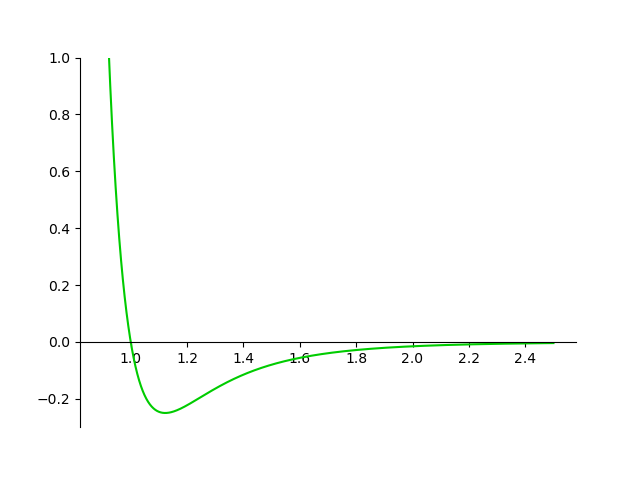
\includegraphics[width=\columnwidth]{./Figures/LJ_plot.png}
		\caption{Lennard-Jones potential}
		\label{LennardJonesplot}
	\end{figure}
	
	Even in numerical methods some are not applicable in reasonable time, the direct sampling for example can be done for few particles but it become unusable quickly.
	So to sample from the Boltzmann distribution one can consider using Markov chains (random chain of states where the state at step $n$ depends only from the step at $n-1$, some talk about chain without memory). Some of the commonly used Markov Chain Monte Carlo will be discuss later.\\
	To sample a correct distribution the algorithm has to respect the global balance condition \eq{eq: Global Balance}, which state that the probability flow going to a state is equal to the flow going outside of it. An important remark is that for each pair of state the total flow between them can be non zero, when this effective flow is zero we respect a condition that is more restrictive than the global balance, the local balance \eq{eq: Local Balance}. This condition are highly related to the method chose for the implementation. As shown in \eq{eq: Flow}, the flow is express thanks to the transfer matrix $\probb{j,i}$ of the process, which give the probability to switch from state j to state i.
	\begin{equation}
		\label{eq: Flow}
		\FCAL \glb j , i \grb = \pi \glb j \grb \probb{j,i}
	\end{equation}
	\begin{equation}
		\label{eq: Global Balance}
		\sum\limits_{j} \FCAL \glb j , i \grb = \sum\limits_{j} \FCAL \glb i , j \grb
	\end{equation}
	\begin{equation}
		\label{eq: Local Balance}
		\FCAL \glb j , i \grb = \FCAL \glb i , j \grb
	\end{equation}
	
	For rest of the discussion we aim to compare time complexity of different algorithms as functions of the number of particle in interaction denoted $\Npart$.
	
	\section{The commonly used Algorithms}
	In this first part we will discuss some algorithms that can be used to sample Lennard-Jones systems starting from the most simple algorithm the Metropolis Monte Carlo \prog{Metropolis}. In one one step, a move $\deplb{X}{X'}$ is proposed with an a priori probability and is accepted with the probability $\prob^{Met}\glb X, X'\grb$ given in \eq{eq : Metropolis}, in which $\pi$ is the Boltzmann weight related to the full potential.
	
	\begin{equation}
		\label{eq : Metropolis}
		\prob^{Met}\glb X, X'\grb = \minc{1, \fracb{\pi \glb X'\grb}{\pi \glb X\grb}}
	\end{equation}
	
	\begin{algorithm}[htb]
		\newcommand{\algo}{Metropolis}
		\captionsetup{margin=0pt,justification=raggedright}
		\begin{center}
			$\begin{array}{ll}
				& \PROCEDURE{\algo}\\
				& \INPUT{x}\\
				& \IS{x'}{x}\\
				& \IS{\delta}{\ranb{-1,1}}\\
				& \IS{\Delta U}{U\glb x+\delta \grb - U\glb x \grb }\\
				& \IS{\lambda}{\mind{1, \expc{-\beta \Delta U}}}\\
				& \IS{\Upsilon}{\ranb{0,1}}\\
				& \IF{\Upsilon < \lambda} \IS{x'}{x + \delta}\\
				& \OUTPUT{x'}\\
				& \ENDPROCEDURE\
			\end{array}$
		\end{center}
		\caption{\sub{\algo}.}
		\label{alg:\algo}
	\end{algorithm}
	
	From the definition of Metropolis filter, we can show that this algorithm respect the local balance at one condition, the a priori probability must be symmetric.\\
	From the pseudo code we can see that for each step, the time complexity is given by the time complexity to compute the potential change $\Delta U$. Since we are moving one particle at a time, it can be compute in a time $\OCAL \glb\Npart\grb$ and so it is for one step.\\
		
	The Metropolis algorithm as it is the easiest method will be the reference for our comparison in the following.\\
	
	In fact Metropolis method is one of the elementary bricks for the Multiple Time Step Monte Carlo \prog{MTSMC} presented by Berne and Hetényi in \cite{Berne2002}. MTSMC also work with the factorization of the potential $U$ in two part $U_I$ and $U_{II}$.
	In their paper they distinguish $U_I$ and $U_{II}$ as a rapidly changing potential and a slow changing one. The first term is used to compute the proposed moved by doing a Metropolis chain of $n$ steps using the Boltzmann weights derived from $U_I$, the resulting position is then accepted with the Metropolis filter for the slow changing potential. In the case of the Lennard-Jones potential, $U_I$ is the short range interaction, the potential truncated at the radius $r_s$ and $U_{II}$ is the far range contribution(the potential above $r_s$).
	
	\begin{algorithm}[htb]
		\newcommand{\algo}{MTSMC}
		\captionsetup{margin=0pt,justification=raggedright}
		\begin{center}
			$\begin{array}{ll}
				& \PROCEDURE{\algo}\\
				& \INPUT{x}\\
				& \IS{x'}{x} \\
				& \IS{y}{x} \\
				& \FOR {i = 0,...,n-1}\\
				& \BRACE{\IS{\delta}{\ranb{-1,1}}\\
					\IS{\Delta \Ufast}{\Ufast\glb y + \delta \grb - \Ufast\glb y \grb } \\
					\lambda = \mind{1,\expc{-\beta \Delta \Ufast}}\\
					\IS{\Upsilon}{\ranb{0,1}}\\
					\IF{\Upsilon < \lambda} \ \IS{y}{y + \delta} 
				}\\
				& \IS{\Delta \Uslow}{\Uslow\glb y \grb - \Uslow\glb x \grb } \\
				&\lambda = \mind{1,\expc{-\beta \Delta \Uslow}}\\
				&\IS{\Upsilon}{\ranb{0,1}}\\
				&\IF{\Upsilon < \lambda} \ \IS{x'}{y} \\
				& \OUTPUT{x'}\\
				& \ENDPROCEDURE\
			\end{array}$
		\end{center}
		\caption{\sub{\algo}, One single step between two sample point}
		\label{alg:\algo}
	\end{algorithm}
	
	As shown in \cite{Berne2002}, this algorithm respect local balance between the end points of the short range chain. Note that it is not possible to sample point during the short range step without inducing bias in the sampling and resulting on a non correct algorithm. One can also question the pertinence of doing the small chain as it is clear that we keep a time complexity $\OCAL\glb\Npart\grb$.\\
	In their paper they achieve to show a CPU time speedup, they also adjust their raw time with a diffusion coefficient using similar methods as in \cite{Rao1979}. MTSMC is so almost 5 time faster than what we can expect to be a Metropolis in their paper.\\
	
	Both previous algorithm rely on proposed move than is accepted or refused, with principle of consensus, we can factorize the problem and work with wisely choose and work with the Boolean variable (instead of multiplying the probabilities together, we will accepted the move if it is accepted for all the terms separately). It can be resume with the following truth table.
	
	\begin{displaymath}
		\begin{array}{|c c|c}
			U_I & U_{II} & U_I + U_{II}\\
			\hline
			\text{Refused} & \text{Refused} & \text{Refused}\\
			\text{Refused} & \text{Accepted} & \text{Refused}\\
			\text{Accepted} & \text{Refused} & \text{Refused}\\
			\text{Accepted} & \text{Accepted} & \text{Accepted}
		\end{array}
	\end{displaymath}
	
	Pushing the consensus idea with lifting the motion (the direction of the motion is fixed and is re-sampled once in a while) we can then work with piece wise deterministic simulation. This is the essence of Event Chain Monte Carlo (ECMC). \\
	To explain  it, let consider one particle moving along positive x direction interacting with one single other particle (going to multiple particles will be simple considering the consensus principle). Let note that the direction being fixed, the potential seen by the moving particle is not the one given in \fig{LennardJonesplot} but will be more like in  \fig{LennardJonesseen}.
	
	\begin{figure}[htb]
		\centering
		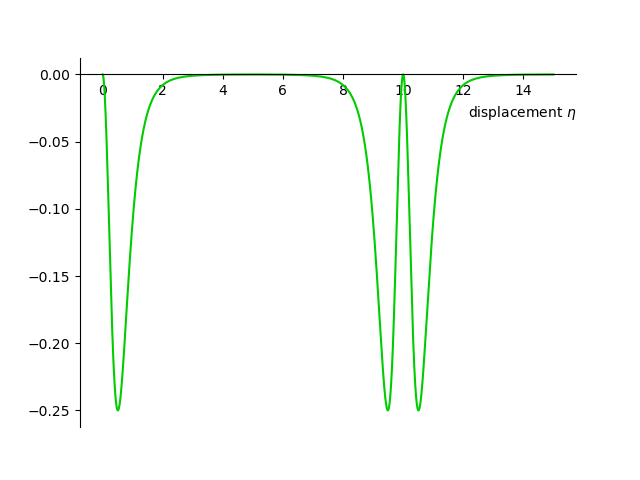
\includegraphics[width=\columnwidth]{./Figures/LJ_seen.png}
		\caption{Potential seen by a particle moving in a fixed direction along its displacement in a periodic boundary box. Here we have particle moving along x axis at $y=0$ with a second particle (source of the interaction)  at position $(0,1)$}
		\label{LennardJonesseen}
	\end{figure}
	
	In the ECMC method, describe in \cite{Faulkner2018}, the moving particle will make infinitesimal displacement $ds$ until the move is rejected.
	Let consider the particle doing small steps of length $\eta$, the probability to stop at the m-th move is given by $p\glb m\grb = \prod \limits_{k = 1}^{m-1} \expb{-\beta\Delta U^+(k)} (1 - \expb{-\beta\Delta U^+(m)})$ with $\Delta U^+(k) = \maxc{0, \Delta U(k)}$ where $\Delta U(k)$ is the potential change induced by the k-th step.	
	In the limits of $\eta \rightarrow 0$ and by changing from variable m to the total positive potential change $U^+_M$ express in \eq{eq: LJCumulative} (shown in \fig{LJCumulative}), we have the following law $p\glb U^+_M \grb = \beta\expb{-\beta U^+_M}$ and so the potential change to do before the rejection.
	\begin{equation}
		\label{eq: LJcummulative}
		\begin{split}
			U^+_M \glb \eta_M \grb &= \int_{0}^{\eta_M} \maxc{0, \partial_x U (\vec{r} + s \vec{e}_x)} ds\\
			&= \int_{0}^{\eta_M} q_{at}(\vec{r} + s \vec{e}_x) ds
		\end{split}
	\end{equation}
	\begin{figure}[htb]
		\centering
		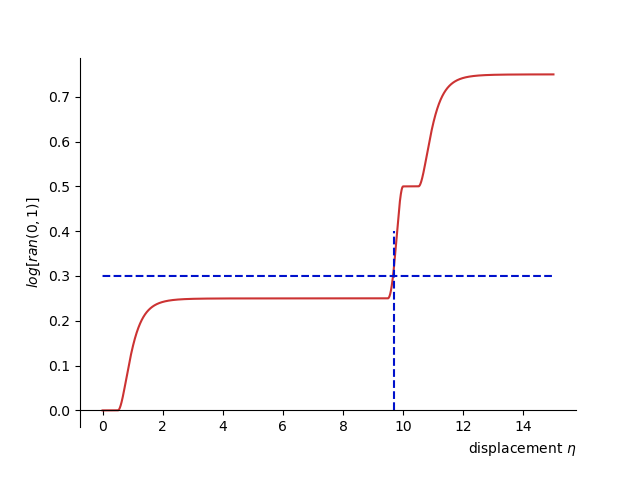
\includegraphics[width=\columnwidth]{./Figures/LJ_cumulative.png}
		\caption{Integration of the rejection which is the potential seen by the particle where we keep the increasing portion of it shifted to keep continuity.}
		\label{LJCumulative}
	\end{figure}
	
	To complete the ECMC process we then need to invert the cumulative rejection rate. This cannot be done by an analytic formula due to the periodicity of property of the system. Some methods can be implemented to compute the needed displacement. \\
	The first one is the straight forward method, we will displace the particle by small steps $\Delta s$, will add up the positive potential change through the displacement and finally stop when we reach the wanted cumulative rejection rate. This methods has has two flaws, the total displacement is given with an accuracy of $\Delta s$ and it is particularly slow for particles highly separated.\\
	For our second method, we will inspire from the method used in JeLLyFysh (JF) \cite{Hoellmer2020} to inverted the real Lennard-Jones potential. We adjust the inverting function in the potential python class to take in account the periodicity. This methods are $findDisplacement$ in \alg{ECMC}\\
	We then have our piece to complete the ECMC procedure for more than two particle. Note that we will make event chain of fixed length and sample only the ending of each chain (even if we can sample more points in the chains).
	\begin{algorithm}[htb]
		\newcommand{\algo}{ECMC}
		\captionsetup{margin=0pt,justification=raggedright}
		\begin{center}
			$\begin{array}{ll}
				& \PROCEDURE{\algo}\\
				& \INPUT{X}\\
				& \IS{a}{\CHOICE{particles}}\\
				& \IS{dir}{\CHOICE{\VEC{e_x},\VEC{e_y}}}\\
				& \IS{Todo}{ChainLength}\\
				& \WHILE{ToDo > 0}\\
				& \BRACE{
					\IS{Ds}{ToDo}; \IS{nextPart}{a}\\
					\IS{\Delta U^+}{-\logc{\ranb{0,1}}}\\
					\FOR{target = particles \neq a}\\
					\BRACE{
						\IS{\Delta s}{findDisplacement\glb a,target,\Delta U^+\grb}\\
						\IF{\Delta s < Ds}\\
						\BRACE{
							\IS{Ds}{\Delta s}\\
							\IS{nextPart}{target}
						}\\
					}\\
					\IS{X}{DoDisplacement(X,a,Ds)}
					\IS{ToDo}{ToDo - Ds}\\
					\IS{a}{nextPart}
				}\\
				& \OUTPUT{X}\\
				& \ENDPROCEDURE\
			\end{array}$
		\end{center}
		\caption{\sub{\algo}. Where X is ca configuration of particles positions that will be updated by the procedure}
		\label{alg:\algo}
	\end{algorithm}
	
	So to have the procedure from the two particles methods, we just have to do it for the possible pairs involving the chosen moving particle. To ensure the consensus along the chain, we then keep the lowest displacement and change the active particle for the one triggering the event. One can discuss what happen if two different particles trigger an event at the same time but those type of event are especially rare and since ce are working with numerical number, the space is discrete.\\
	
	This algorithm still have a time complexity of $\OCAL \glb \Npart\grb$ per step, with steps that can be particularly slow. So what is the point of presenting it? This algorithm will be use as a step to the last algorithm that will be discuss here, the Cell Veto Monte Carlo (CVMC) but first let make a small check point and see if all the three algorithms already presented have compatible results.
	
	\begin{table}[htb]
		\begin{tabular}{|c|c|c|}
			\hline
			 & mean Separation & standard deviation\\
			 \hline
			 Metropolis & 3.89147 & 0.00429\\
			 MTSMC & 3.88850 & 0.00284\\
			 ECMC & 3.89148 & 0.00992\\
			 \hline
		\end{tabular}
		\caption{Mean separation between pair of particles obtain for 100 runs of $10^5$ steps for each algorithm. We run  the algorithms with 4 particles in a periodic box of size $L=10$ with an inverse temperature $\beta = 1$. The MTSMC parameter was $n=4$ and the ECMC chain length was $1.0$. Finally for the MTSMC and the Metropolis, the step size was taken with a uniform distribution in $\glc 0,1 \grc$}
		\label{partialComparison}
	\end{table}
	 
	We can see that those three algorithm have compatible results. Note that it is note given with the best precision, more runs of each algorithm will be needed to have a more accurate value of  the mean separation.
	
	
	\section{Cell-veto}
	We have presented three algorithm that can sample a Lennard-Jones system, they all have a time complexity of $\OCAL\glb\Npart\grb$ per step and so share the problem to not have the possibility to sample a system where many particle interact. We will here describe an algorithm based on the ECMC that can be implemented with a time complexity $\OCAL\glb 1 \grb$.\\
	Firstly introduce S.C.Kapfer and W.Krauth in \cite{KapferKrauth2016}, the cell veto algorithm \alg{Cell-Veto} is based on ECMC but the event will at first be trigger at cell level and then be verified as a true or a fake event.
	
	\begin{figure}[htb]
		\centering
		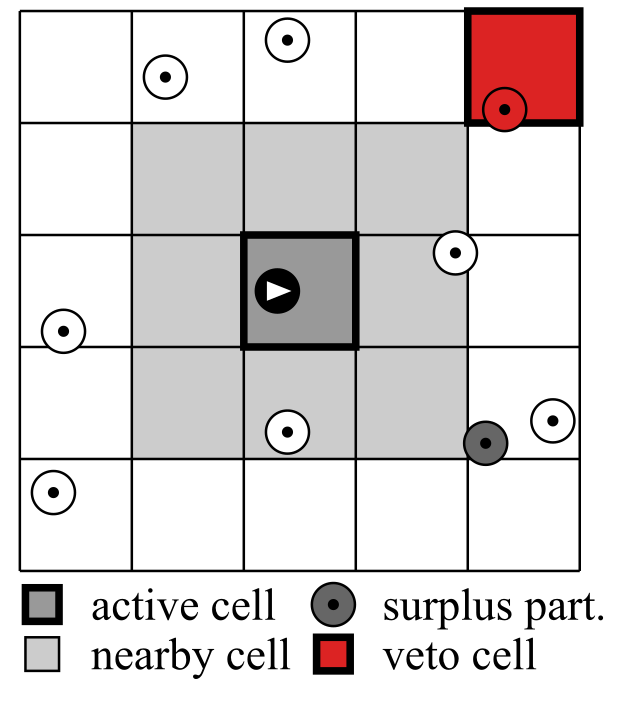
\includegraphics[width=0.7\columnwidth]{./Figures/CellVetoSchema.png}
		\caption{Image extract from \cite{KapferKrauth2016} to explain the Cell Veto algorithm. The events are trigger at cells level with a bounding event rate for each possible target cell with the active cell, the event is than confirmed at the particle level in the vetoing cell. Neighboring cells and surplus are treated separately.}
		\label{CVSchema}
	\end{figure}
	
	The far field is then treated with a bounding potential (a potential for which the derivative along the chosen direction is always bigger than the derivative of the actual potential). In our case, we will have a piece wise linear bounding potential, ie. the derivative of the bounding potential will be constant on a cell.\\
	
	To accept it as a true or a fake event one need to compare the event rate at a cell level $Q_{at}$  with the one at particle level $q(\vec{r}_{at})$. If a particle exist in the triggering cell, the event is accepted with a probability $\fracb{q(\vec{r}_{at})}{Q_{at}}$ \fig{derivativeMethod}.\\ 
	
	\begin{figure}[h!]
		\centering
		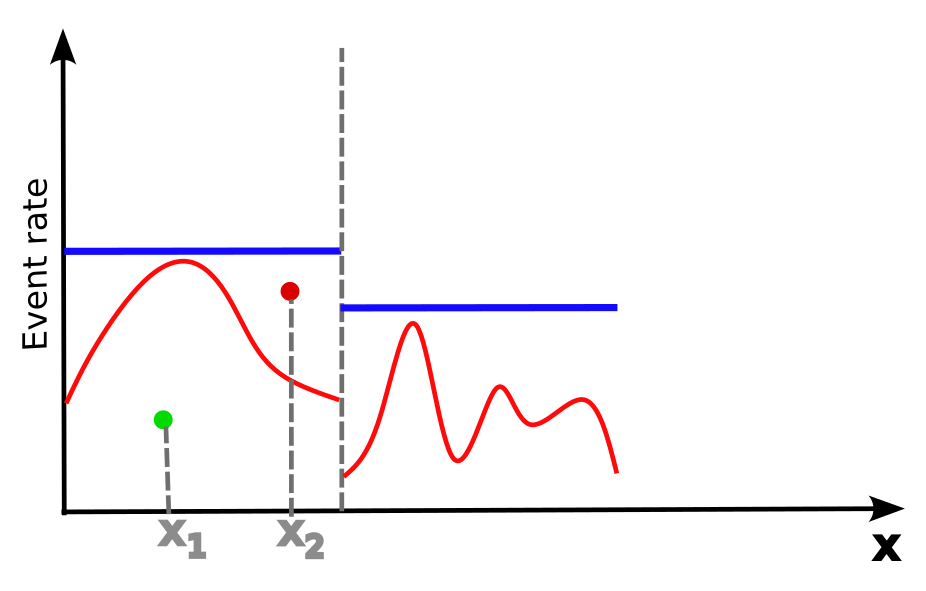
\includegraphics[width=0.9\columnwidth]{./Figures/DerivativeMethod.png}
		\caption{In this schema, the blue line is the bounding potential event rate and the red line correspond to the one of the actual potential. In the derivative method, a displacement is sample thanks to the bounding potential (x1 or x2). Then the position below the blue line is sample randomly, it is consider a true event when it is below the red line (like the green point), if the point is above, the event is a fake one..}
		\label{derivativeMethod}
	\end{figure}
	
	\begin{algorithm}[htb]
		\newcommand{\algo}{Cell-Veto}
		\captionsetup{margin=0pt,justification=raggedright}
		\begin{center}
			$\begin{array}{ll}
				& \PROCEDURE{\algo}\\
				& \INPUT{X}\\
				& \IS{a}{\CHOICE{particles}}\\
				& \IS{dir}{\CHOICE{\VEC{e_x},\VEC{e_y}}}\\
				& \IS{Todo}{ChainLength}\\
				& \WHILE{Todo > 0}\\
				& \BRACE{
					\IS{ds}{Todo}\\
					\IF{FrontierDistance < ds} \IS{ds}{FrontierDistance}\\
					\IS{\Delta s}{-\fraca{\logc{\ranb{0, 1}}}{Q_{tot}}}\\
					\WHILE{\Delta s < ds}\\
					\BRACE{
						\IS{targetCell}{WalkersSampling}\\
						\IF{\ranb{0,1} < \fracb{q(\vec{r}_{at})}{Q_{at}}}\\
						\BRACE{
							\IS{nextPart}{CellOccupant[targetCell]}\\
							\IS{ds}{\Delta s}\\
							\BREAK
						}\\
					\IS{\Delta s}{\Delta s + -\logc{\ranb{0, 1}}}
					}\\
					\IS{\Delta U^+}{-\logc{\ranb{0, 1}}}\\
					\FOR{\text{target in surplus or neighborhood}}\\
					\BRACE{
						\IS{\Delta s}{findDisplacement\glb a,target,\Delta U^+\grb}\\
						\IF{\Delta < ds}\\
						\BRACE{
							\IS{nextPart}{target}\\
							\IS{ds}{\Delta s}
						}\\
					}\\
				}\\
				& \OUTPUT{X}\\
				& \ENDPROCEDURE\
			\end{array}$
		\end{center}
		\caption{\sub{\algo}. As for ECMC, we will sample point at a fixed chain length.}
		\label{alg:\algo}
	\end{algorithm}
	
	The neighboring cells and the surplus particle will be treated individually. The contribution in time will be constant for a given cell size as the number of nearby cells will remain constant. The contribution of the surplus particle is also negligible as we can chose a clever cell size as a function of the particle density to ensure that surplus particles will be very rare.\\
	
	This is enough to ensure a time complexity of $\OCAL\glb N_{cell} \grb$ but we will have $N_{cell} > \Npart$ to ensure the rarity of surplus particle but we are not far from the promise land of a constant time complexity. We will need to have a clever way to select the triggering cell with a known displacement.\\
	
	To fasten the process, we will treat the far field all together instead of each cell separately. We will trigger a possible event at the rate $Q_{tot} = \sum\limits_{target cells} Q_{at}$, this is possible because we consider infinitesimal steps.\\
	
	With this event trigger at the level of the far field, we have to scale down to the cell level, a cell has a probability $\fracb{Q_{at}}{Q_{tot}}$ to be the one triggering the event. We can chose the triggering cell with the tower sampling method \fig{tower sampling}, we consider a tower where each floor is a cell and the height of the floor is $Q_{at}$. With this tower, we sample in this tower with a random number between 0 and $Q_{tot}$ and then we must know in which floor this number fall. This method is straightforward and simple to understand but its implementation lead to a complexity $\OCAL\glb N_{cell} \grb$ in the worst case. It is then needed to find a better method.\\
	
	\begin{figure}[htb]
		\centering
		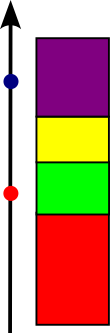
\includegraphics[width=0.18\columnwidth]{./Figures/towerMethod.png}
		\caption{Each color on the tower represent a cell, the height is proportional to the rate $Q_{at}$. The point on the axis are random number used to know which cell trigger the event (Red dot $\rightarrow$ green cell). Note that when red dot value need to be compare only twice, the blue one need to be compare four time}
		\label{tower sampling}
	\end{figure}
	
	The tower sampling being quite slow, we will use the Walker's method \fig{Walker's Method} to find the triggering cell. Instead of working with a tall tower of height $Q_{tot}$, we will make many small towers of height $Q_{mean} = \fraca{Q_{tot}}{N_{cells}}$, and so each tower have the same weight and can be chose uniformly. Each tower will be composite of a maximum of two cells (note that a cell can be represented in more than one tower) at a rate specific for each tower. All the information (rate, first cell, second one) will be stored in a table that is calculated only once.\\
	
	With the table calculated, we have to take to random numbers, an integer to know which tower will be use and a float number between 0 and $Q_{mean}$ to know which cell of the used tower will be used in the end. This way of sampling do not scale with the number of particle nor the number of cells but will use a bit more memory.\\
	
	\begin{figure}[htb]
		\centering
		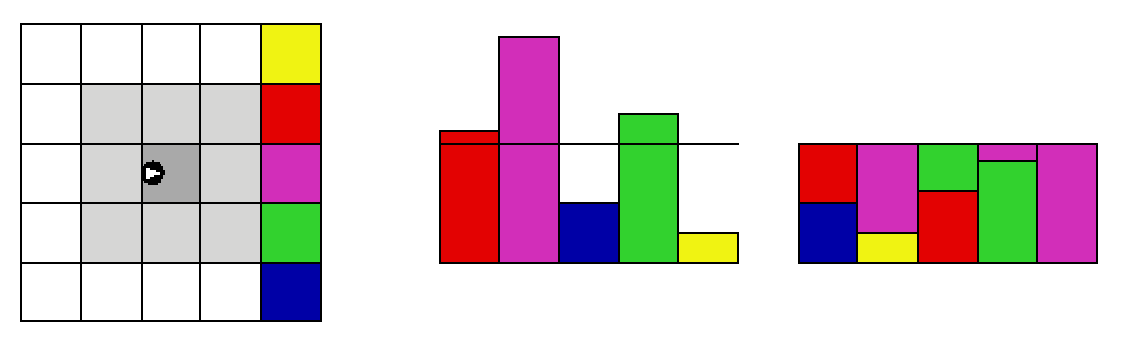
\includegraphics[width=\columnwidth]{./Figures/WalkerMethod.png}
		\caption{\textbf{Left:} Cells in the far field must have finite rate; \textbf{Center:} Histogram of the five colored cell rate, the mean is indicated by the vertical bar; \textbf{Right:} The composites of height $Q_{mean}$ composed of at most two cells}
		\label{Walker's Method}
	\end{figure}

	The far field treatment of Cell Veto Method \alg{Cell-Veto} can be implemented with a constant time complexity. We will work with a fixed chain length. It is also important to note that a pseudo-event (event only not trigger by the potential) will be use when the boundary of a cell is cross because we have to change the active cell.
	
		\begin{table}[htb]
		\begin{tabular}{|c|c|c|}
			\hline
			& mean Separation & standard deviation\\
			\hline
			Metropolis & 3.89147 & 0.00429\\
			MTSMC & 3.88850 & 0.00284\\
			ECMC & 3.89148 & 0.00992\\
			CVMC & 3.88933 & 0.01113\\
			\hline
		\end{tabular}
		\caption{Mean separation between pair of particles obtain for 100 runs of $10^5$ steps for each algorithm. We run  the algorithms with 4 particles in a periodic box of size $L=10$ with an inverse temperature $\beta = 1$. CVMC chain length used was $1.0$ and the cell size $2.0$}
		\label{Comparison}
	\end{table}
	
	The table \ref{Comparison} show that CVMC have compatible result but with more variability.
	
	\section{Perspectives and continuation}
	We have describe and analyze the theoretical time complexity of four algorithms that can be used to sample Lennard Jones system. We still have to run the different algorithms with execution time computation for different values of $\Npart$. In fact it has be done on buggy version of the implementation \fig{time Metropolis} and  \fig{time CVMC}, even if only small change were made, it is important to redo the graphics with the actual implementation of the algorithm.
	\begin{figure}[htb]
		\centering
		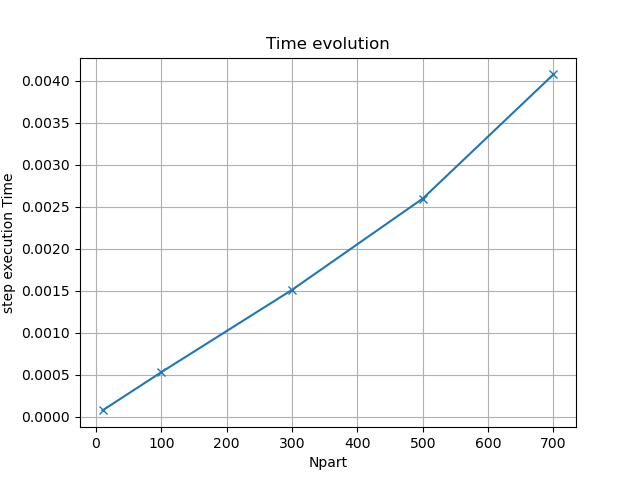
\includegraphics[width=0.8\columnwidth]{./Figures/timeEvolutionMetropolis.png}
		\caption{Mean execution time per step against the number of particles in interaction. \textbf{Important:} This was obtain on an early version of the implementation and may differ a bit for the actual implementation}
		\label{time Metropolis}
	\end{figure}
	
	\begin{figure}[htb]
		\centering
		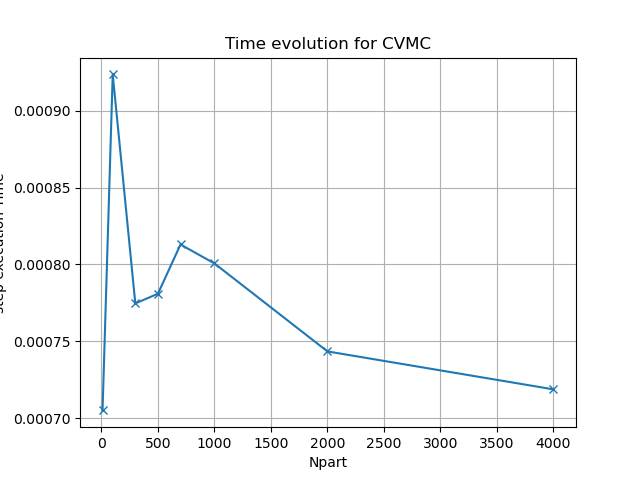
\includegraphics[width=0.8\columnwidth]{./Figures/timeEvolutionCVMC.png}
		\caption{Mean execution time per step against the number of particles in interaction. \textbf{Important:} This was obtain on an early version of the implementation and may differ a bit for the actual implementation}
		\label{time CVMC}
	\end{figure}
	
	Since only small modifications were made, we can expect a similar result for the final implementation.
	From this early investigation, we see that the raw execution times give results compatible with the theoretical ones discuss previously, but raw time are not totally comparable as an algorithm can be slower per step but converge much faster.\\
	
	\newpage
	A way to compare and adjust the time execution must be explore. A possibility is to do as Hetènyi and Berne in \cite{Berne2002}, we can adjust by diffusion but event chain and cell veto has some ballistic component and so the adjustment will be bias in there favor. We must then find a way to compare the convergence of the algorithms.\\
	
	This is the first continuation to the work already done. We can also discuss the optimal parameter for the cell veto, for a given particle density what is the best size for each cell. Here we worked with a grid of identical cells but in fact it is possible to work with cells of different size, for example we can increase the size of cells really far away. One can also optimize the length of the neighborhood since it is what give the number of particles that will be treated differently.\\
	
	To conclude, the cell veto having a constant time complexity open the door to computation not done before due to unreasonable time need to run. One can think of system with to types of particles interacting with different intensities event different interactions can be implemented, this is possible in JeLLyFysh.
	
	\bibliographystyle{ieeetr}
	\bibliography{./Utilities/General.bib,./Utilities/LennardJones.bib}
	
\end{document}